%%%% main.tex
%%%% Course preprint, written in the IJCAI--ECAI 26 style using the official
%%%% author kit (ijcai26.sty, named.bst). This preprint has NOT been submitted
%%%% to IJCAI, and IJCAI has NOT accepted it. The style file is used because
%%%% the assignment asks for it.

\documentclass{article}
\pdfpagewidth=8.5in
\pdfpageheight=11in

\usepackage{ijcai26}

\usepackage{times}
\usepackage{url}
\usepackage[hidelinks]{hyperref}
\usepackage[utf8]{inputenc}
\usepackage[small]{caption}
\usepackage{graphicx}
\usepackage{amsmath}
\usepackage{amsthm}
\usepackage{booktabs}

\urlstyle{same}

% ---------------------------------------------------------------------------
% EDIT THIS ONE LINE: paste the public URL of your repository.
\newcommand{\repourl}{https://github.com/kishore461/ecommerce-review-moderator-agent}
% ---------------------------------------------------------------------------

\pdfinfo{
/TemplateVersion (IJCAI.2026.0)
}

\title{Deciding What to Do With a Review You Cannot Verify:\\
A Cost-Sensitive Belief Agent Using Text and Star Rating Only}

\author{
    Jayakishore
    \affiliations
    Week 1 AI-Native Shipping Sprint
    \emails
    jayakishore2004@gmail.com
}

\begin{document}

\maketitle

\begin{abstract}
    An e-commerce moderation agent observes a newly submitted review's text and
    star rating and must permit, flag, route to a human, or hide it, without
    knowing whether the review is a genuine customer experience, a paid or
    machine-generated fake, or a non-independent review written by someone
    close to the business. We build a small agent that maintains an explicit
    belief over those three hidden states --- though the third carries zero prior
    mass in the main experiment, which is therefore a two-state problem --- and
    selects an action by minimising expected cost under an asymmetric, volume-weighted cost matrix. We compare
    it against a keyword baseline and against a fixed-threshold version of
    itself on a 40-case held-out set and a 12-case adversarial probe set. The
    agent improves precision from 0.647 to 0.933 and recall from 0.550 to
    0.700 on the like-for-like accounting (0.778 if the cases it declines to
    decide are dropped from the denominator), but the result does not survive
    scrutiny intact: the baseline beats
    the agent on the probe set (recall 0.857 versus 0.333), the agent is
    poorly calibrated (ECE 0.145), an ablation shows the six hand-designed
    features contribute a single case beyond the lexical channel, and the
    ranking of the two policies reverses depending on whether routed cases are
    counted. Six design decisions came out of four public discussion threads with
    practitioners and changed the agent in ways the measurements did not,
    including the addition of the third hidden state. We report the negative findings in full because they are the
    informative part.
\end{abstract}

% ===========================================================================
\section{Introduction}

A platform receives a review. It has, at that instant, two things: some text
and a number of stars. It does not have the reviewer's purchase history, IP
address, account age, or photo metadata --- either because the reviewer is new,
or because the platform is small, or because the decision has to be made before
those signals are joined. It must nonetheless do something with the review.

Stated in the form the assignment requires:

\begin{quote}
    The agent observes a newly submitted customer review text and star rating.
    It must select permit, warn, hide, or report because whether the post is a
    genuine customer experience versus a paid spam or competitor fake review is
    not known.
\end{quote}

The constraint --- text and rating, nothing else --- is deliberate and is
enforced in code: the agent's entry point takes \texttt{(text, rating)} and no
other argument. It is also the constraint a practitioner immediately objected
to. In r/LanguageTechnology, u/Mundane\_Ad8936 stated that a single review
cannot be classified without user history or graph features. We agree, and the
project is scoped accordingly: this is a cold-start triage filter whose most
important output is often the admission that it does not know.

This preprint's contribution is not a detector. It is a decision procedure
under a belief, plus an honest account of where that procedure fails. The
findings we consider most useful are negative:

\begin{enumerate}
    \item The agent beats a keyword baseline on held-out data and loses to it
          on a probe set designed to attack its assumptions.
    \item Its beliefs are not calibrated (ECE 0.145), and 60\% of them are
          pinned by a clipping constant rather than by evidence.
    \item The six interpretable features that motivate the whole design
          contribute one case out of forty beyond a plain unigram channel.
    \item Which of the two policies is ``better'' depends entirely on whether
          the cases it declined to decide are counted in the denominator.
\end{enumerate}

\section{Related Work and User Discussions}\label{sec:related}

\paragraph{Prior work.}
Ott et al.~\shortcite{ott2011finding} established that deceptive opinion spam
is separable from genuine review text by psycholinguistic and $n$-gram
features, and produced the first gold-standard deceptive review corpus. Their
positive class is crowdworker-authored deception. Salminen et
al.~\shortcite{salminen2022creating} produced the corpus used here, in which
the positive class is GPT-2-generated review text paired with genuine Amazon
reviews drawn from the corpus of Ni et
al.~\shortcite{ni2019justifying}. Elkan~\shortcite{elkan2001foundations} gives
the decision-theoretic result this agent's policy rests on: with a known cost
matrix, the optimal action is the one minimising expected cost under the
posterior, and thresholds on probability are a special case rather than the
general rule. Guo et al.~\shortcite{guo2017calibration} is the source of the
expected-calibration-error estimator we report and of the observation that a
confident classifier is not thereby a calibrated one. Sap et
al.~\shortcite{sap2019risk} document that lexical classifiers in content
moderation systematically penalise African-American English; we cite it because
it names an untested risk in this system, not because we tested for it.

\paragraph{Discussions with people.}
Six design decisions in this agent came from four public discussion threads
rather than from the literature or from measurement (\texttt{discussion-record.md}
records ten changes in total; these are the six that reach the code). Each is recorded with a link in
\texttt{discussion-record.md}.

\begin{itemize}
    \item \textbf{Probability bands.} Practitioners in r/trustandsafetypros
          described ``warn'' as soft friction or a queue router rather than a
          public label, and put autonomous removal behind high confidence. The
          policy was rewritten as explicit bands: permit below 0.50, human
          queue 0.50--0.84, act at 0.85 and above.
    \item \textbf{Flag instead of hide.} A seller in r/Amazonsellercentral
          objected to autonomous hiding and preferred a flag carrying an
          explanation for manual approval. Policy A's high-confidence action
          was changed accordingly.
    \item \textbf{Volume-weighted costs.} A commenter in r/Yelp stated that the
          damage from a wrongly removed review depends on how many reviews the
          business already has. Every cost of acting wrongly against a genuine
          review, or against a \texttt{solicited} one, is now multiplied by
          $v = \min(1, 200/\text{total\_reviews})$.
    \item \textbf{Specificity over sentiment.} Two r/Yelp users independently
          said a genuinely angry customer names falsifiable detail --- a dish,
          a quantity, a sequence --- while a planted review stays vague. The
          agent's strongest hand-designed feature keys on this, and star/text
          mismatch was demoted to a secondary signal.
    \item \textbf{Specificity qualified.} The same user then said fakers lift
          dish and staff names from the reviews already on the page.
          Specificity separates lazy fakes from real reviews and fails against
          motivated ones. It is reported as non-robust rather than as a
          solution.
    \item \textbf{A third hidden state.} u/ADrPepperGuy clarified that by
          ``fake'' he meant a friend or family member writing a review for
          someone they know. The visit happened and the detail is true, so the
          specificity signal is blind to it by construction. The state
          \texttt{solicited} was added for this reason.
\end{itemize}

\section{Agent Design}

\paragraph{Input.} A review's text and its star rating. Nothing else.

\paragraph{Hidden states.}
$\mathcal{S} = \{\texttt{genuine}, \texttt{fake}, \texttt{solicited}\}$:
an independent customer; a paid, competitor, or machine-generated review; and a
review by someone with a personal relationship to the business, whose visit was
real but whose review is not independent.

\paragraph{Belief.} A full posterior over $\mathcal{S}$, not a score.

\paragraph{Actions.}
$\mathcal{A} = \{\texttt{permit}, \texttt{flag}, \texttt{route},
\texttt{hide}\}$, written in full as \texttt{flag\_with\_explanation} and
\texttt{route\_to\_human} in the code. These realise the assignment's
permit/warn/hide/report: \texttt{flag} is the warn action
and \texttt{route} is the report action, both named after the form
the r/trustandsafetypros practitioners described.

\paragraph{Human reasoning function.}
One only: identify uncertainty and hand a high-cost decision to a person rather
than guessing. Both policies may decline to decide. No other human faculty is
imitated.

\paragraph{Evidence channels.}
Six discrete interpretable features are extracted from text and rating:
\texttt{specificity} (3 levels), \texttt{generic\_praise} (3),
\texttt{length\_band} (4), \texttt{polarity\_mismatch} (2),
\texttt{experience} (2), \texttt{exclamation} (3). Separately, a unigram Naive
Bayes channel is fit on a 6{,}000-row training split (vocabulary 3{,}835 terms
after a minimum document frequency of 5), producing a log-likelihood ratio that
is clipped at $\pm4.0$.

\paragraph{Feedback.}
\texttt{FeedbackLog} records human verdicts for cases sent to the queue and for
enforcement actions that are later appealed. Permitted reviews generate
nothing, which is a structural limitation identified in r/learnmachinelearning
and discussed in Section~\ref{sec:limits}.

\section{Probability Model and Decision Rule}

\subsection{Belief update}

Let $f_1,\dots,f_6$ be the observed feature levels and $w_1,\dots,w_n$ the
review's in-vocabulary tokens. Treating the channels as conditionally
independent given the state,
\begin{equation}
    P(s \mid f, w) \;\propto\; P(s)\prod_{i=1}^{6}P(f_i \mid s)\cdot
    \exp\!\big(\lambda_s(w)\big),
    \label{eq:posterior}
\end{equation}
computed in log space. The feature likelihoods $P(f_i \mid s)$ are estimated on
the training split with Laplace smoothing:
\begin{equation}
    P(f_i = \ell \mid s) = \frac{c_s(f_i = \ell) + 1}{c_s + L_i},
\end{equation}
where $L_i$ is the number of levels of feature $i$. This holds for
\texttt{genuine} and \texttt{fake} only. The \texttt{solicited} row is not
fitted: five of its six features are copied from \texttt{genuine} and
\texttt{generic\_praise} is reweighted toward heavier praise by a stipulated
factor (\texttt{SOLICITED\_ASSUMPTION} in the code). The lexical term is the
clipped log-likelihood ratio
\begin{equation}
\begin{split}
    \lambda_s(w) &= \mathrm{clip}\big(\Lambda(w),\,-\tau,\,\tau\big),
    \quad \tau = 4.0,\\
    \Lambda(w)   &= \sum_{j=1}^{n}
    \log\frac{P(w_j \mid \texttt{fake})}{P(w_j \mid \texttt{genuine})},
\end{split}
    \label{eq:llr}
\end{equation}
added with sign $+$ for \texttt{fake} and set to exactly $0$ for both
\texttt{genuine} (the reference state) and \texttt{solicited}. The lexical
channel therefore contributes $\Lambda$, not $2\Lambda$, to the
fake-versus-genuine log-odds, and contributes nothing at all to
\texttt{solicited} --- an admission of ignorance whose consequence we quantify
in Section~\ref{sec:limits}.

The quantity both policies act on is
$p = P(\texttt{fake}) + P(\texttt{solicited})$.

\subsection{Cost matrix}

Costs are in relative units. With volume factor
$v=\min(1,\,200/\text{total\_reviews})$:

\begin{center}
\small
\begin{tabular}{lccc}
\toprule
Action & \texttt{genuine} & \texttt{fake} & \texttt{solicited} \\
\midrule
\texttt{permit} & $0$    & $5$ & $2$ \\
\texttt{route}  & $1$    & $1$ & $1$ \\
\texttt{flag}   & $2v$   & $1$ & $1.5v$ \\
\texttt{hide}   & $10v$  & $0$ & $6v$ \\
\bottomrule
\end{tabular}
\end{center}

Only the presence of $v$ is evidence-based, from the r/Yelp conversation. The
magnitudes are stipulated; no seller answered the direct question about what a
wrongly removed review costs, across two subreddits and one X post.

\subsection{The two policies}

\textbf{Policy A (fixed bands)} acts on $p$ alone: \texttt{permit} if
$p<0.50$, \texttt{route\_to\_human} if $0.50\le p<0.85$, and
\texttt{flag\_with\_explanation} if $p\ge0.85$. It is never permitted to hide.

\textbf{Policy B (expected cost)} follows Elkan~\shortcite{elkan2001foundations}
and selects
\begin{equation}
    a^\star = \arg\min_{a\in\mathcal{A}}\;
    \sum_{s\in\mathcal{S}} P(s \mid f, w)\, C(a, s),
    \label{eq:argmin}
\end{equation}
with ties broken toward the least destructive action
(\texttt{permit} $<$ \texttt{route} $<$ \texttt{flag} $<$ \texttt{hide}) and the
tie noted in the decision reason. Policy B may hide.

Comparing A with B was intended as a direct test of the design change made
after the r/Amazonsellercentral discussion. It is not one. Under this cost
matrix \texttt{flag} is weakly dominated by \texttt{route} for every belief, so
Policy B never flags --- zero flags on both datasets --- and its only
enforcement action is hiding. The comparison confounds two changes:
threshold-versus-cost, and flag-only-versus-hide-only.

\section{Test Method}

\paragraph{Data.} The Fake Reviews Dataset of Salminen et
al.~\shortcite{salminen2022creating}, 40{,}432 rows labelled \texttt{CG}
(computer-generated) and \texttt{OR} (original human). Splitting is
deterministic under seed 20260817 into a 6{,}000-row fit split and a 40-case
held-out test set balanced 20/20.

\paragraph{Labelling provenance.} This is stated explicitly because a
r/learnmachinelearning commenter asked for it. The test-set labels are the
dataset's own \texttt{CG}/\texttt{OR} labels, decided by the dataset authors'
construction procedure, not by us. The 12-case probe set is hand-written by the
author, and its labels are the author's by construction --- which is why it is
reported separately and never pooled with the 40.

\paragraph{Probe set.} Twelve cases written to attack specific assumptions:
solicited reviews with true detail, fakes with detail harvested from a product
page, sarcasm with inverted polarity, and terse genuine reviews. It runs under
a different prior (0.60/0.30/0.10) because \texttt{solicited} has zero prior
mass in the main run and cannot otherwise be inferred; probe and test numbers
are therefore not directly comparable.

\paragraph{Baseline.} A flat keyword rule with no belief, no cost model, and no
option to defer. Its term-count threshold is tuned on the fit split to maximise
$F_1$ (tuned value 1). Its keyword list was generated with LLM
assistance, following a suggestion in r/learnmachinelearning. It cannot settle
the follow-up question we asked there --- whether LLM-generated rules inflate
false positives --- because there is no hand-written control list to compare
against; the lexical-only ablation row serves as the stronger comparator
instead.

\paragraph{Metrics.} Precision and recall against the positive class
``not genuine''; expected calibration error over five equal-width bins
following Guo et al.~\shortcite{guo2017calibration}; total cost under the cost
matrix; and the human-review rate. Two recall figures are reported throughout,
excluding and including routed cases in the denominator, for reasons given in
Section~\ref{sec:results}.

\paragraph{Reproduction.} Three seeded commands, Python 3.11, no third-party
packages (the figure script uses matplotlib), no network. The seventeen
parameters in \texttt{results/run\_manifest.json} cover the splits, priors,
thresholds and lexical settings; the two smoothing constants, the
\texttt{solicited} reweighting factors and the cost magnitudes live in the
source and are not in the manifest. The source dataset is not checksummed, so
the numbers reproduce exactly against the same download and are not guaranteed
against a re-download. Code: \url{\repourl}.

\section{Results}\label{sec:results}

\begin{table}[t]
\centering
\small
\begin{tabular}{lccccc}
\toprule
System & Prec. & Rec. & Rec.$^\dagger$ & Cost & ECE \\
\midrule
baseline\_keyword & 0.647 & 0.550 & 0.550 & 68.0 & n/a \\
fixed\_band (A)   & 0.933 & 0.778 & \textbf{0.700} & 42.0 & 0.145 \\
expected\_cost (B)& 0.929 & 0.867 & 0.650 & 31.0 & 0.145 \\
\bottomrule
\end{tabular}
\caption{Held-out test set, 40 cases (20 genuine / 20 fake).
$\dagger$ counts routed cases in the denominator. Human-review rate: 0\%,
15.0\%, 27.5\%. The cost column is reported but is not a valid comparison ---
see the text.}
\label{tab:main}
\end{table}

\begin{figure*}[t]
\centering
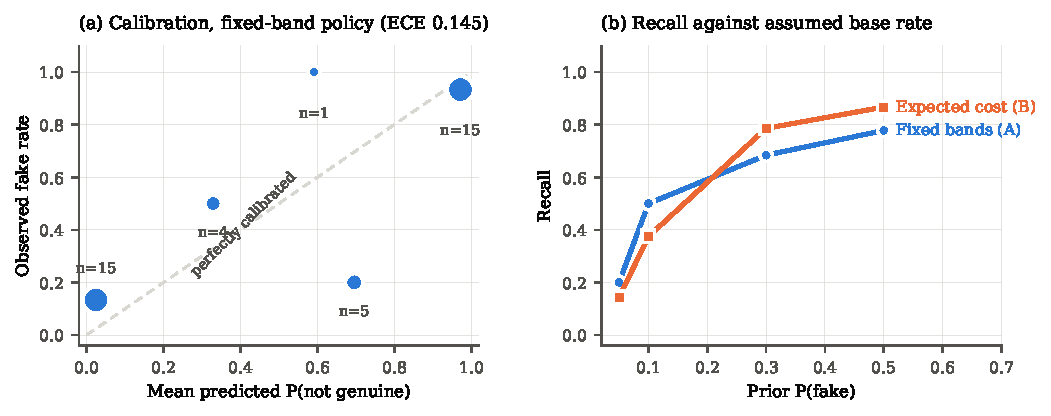
\includegraphics[width=0.74\textwidth]{figures/figure1.pdf}
\caption{(a) Reliability of the agent's beliefs on the held-out set; marker
area is proportional to bin count. The $[0.6,0.8)$ bin sits far below the
diagonal but holds five cases. (b) Recall against the assumed base rate. Both
policies degrade sharply as $P(\texttt{fake})$ falls toward a realistic
deployment value.}
\label{fig:main}
\end{figure*}

Both agent policies beat the baseline on precision and recall on the held-out
set. Four qualifications apply, and they are the substance of this section.

\paragraph{The cost comparison is circular.} Policy B selects the action
minimising expected cost under a cost model and is then scored with that same
cost model. ``B has the lowest cost'' is a property of
Equation~\eqref{eq:argmin}, not a finding. The column is printed for
completeness and excluded from every claim.

\paragraph{The policy ranking reverses.} Excluding routed cases from the
denominator flatters a policy that declines --- an agent routing 39 of 40 cases
and getting the last one right would score perfectly. Including them penalises
a policy for correctly identifying its own uncertainty, and the baseline cannot
route at all, so only that version is like-for-like. Under the first, B leads
(0.867 vs.\ 0.778); under the second, A leads (0.700 vs.\ 0.650). We report
both and claim neither policy is better.

\paragraph{The baseline wins on the probe set.} On the 12 hand-written
adversarial cases the baseline reaches recall 0.857 against 0.333 for both
agent policies. The probe set was built to attack the agent's assumptions and
it succeeds.

\paragraph{The features contribute almost nothing.}
Table~\ref{tab:ablation} removes each channel. With the feature terms genuinely
omitted from Equation~\eqref{eq:posterior} --- not set to level zero, which
injects $-1.86$ log-odds and is not removal --- the lexical channel alone
reaches recall 0.765 (A) and 0.867 (B) against 0.778 and 0.867 for the full
system: one true positive on A, none on B. On A they also remove one false
positive (precision 0.933 against 0.867), which is the larger of their two
contributions and is invisible in a recall-only table. Alone they never reach
the acting threshold at all: under Policy A they permit 18 cases and route the
other 22, giving recall 0.000; under Policy B they route all 40. An earlier
version of this work
reported that features raised recall from 0.632 to 0.778; that was an artefact
of the level-zero bug, found in review and corrected.

\begin{table}[t]
\centering
\small
\begin{tabular}{llccccc}
\toprule
Channels & Pol. & TP & FP & FN & Rt. & Prec. / Rec. \\
\midrule
feat.+lex. & A & 14 & 1 & 4 & 6  & 0.933 / 0.778 \\
feat.+lex. & B & 13 & 1 & 2 & 11 & 0.929 / 0.867 \\
lex.\ only & A & 13 & 2 & 4 & 6  & 0.867 / 0.765 \\
lex.\ only & B & 13 & 1 & 2 & 10 & 0.929 / 0.867 \\
feat.\ only & A & 0 & 0 & 5 & 22 & --- / 0.000 \\
feat.\ only & B & 0 & 0 & 0 & 40 & --- / --- \\
\bottomrule
\end{tabular}
\caption{Channel ablation on the held-out set. ``Features only'' under
Policy B routes every case, so it has no decisions to score.}
\label{tab:ablation}
\end{table}

\paragraph{The headline numbers do not travel.} Table~\ref{tab:main} assumes a
50\% base rate of fakes, which no deployment has. Sweeping the prior
(Figure~\ref{fig:main}b) gives recall 0.778 $\rightarrow$ 0.500 $\rightarrow$
0.200 for Policy A and 0.867 $\rightarrow$ 0.375 $\rightarrow$ 0.143 for
Policy B as $P(\texttt{fake})$ falls from 0.5 to 0.1 to 0.05.

\paragraph{Calibration.} ECE is 0.145 on the test set and 0.211 on the probe
set. The $[0.6,0.8)$ bin predicts a mean of 0.696 against an observed rate of
0.200, but holds five cases; bin counts are printed beside every reliability
table for that reason.

\section{Failure Analysis}

Routed cases are not counted as failures --- declining to decide is a permitted
action. \texttt{results/failures.md} names nine failure conditions across the
two datasets; the five largest are described here, and they cover 29 of the 35
incorrect decisions. The counts in parentheses are counts of \emph{incorrect
decisions}, pooled across all three systems, not of distinct cases --- the same
review can be got wrong by more than one system.

\paragraph{SHORT-FAKE-MISSED (9 decisions, 5 cases).} Too little text to separate from a
short genuine review. \emph{``Came broken and cracked frame. The only way to
fix it was to just fix the frame''} --- true state \texttt{fake}, 1 star,
permitted by both the baseline and Policy A at $p=0.339$.

\paragraph{SPECIFIC-GENUINE-FLAGGED (8 decisions, 7 cases).} A detailed real review acted on
anyway. This produces the single most expensive decision in the experiment:
\emph{``My dog loves this toy and is always chewing on it and he has nice
strong, clean teeth. This is my 3rd one''} --- genuine, 4 stars, and Policy B
assigns $p=0.983$ and \emph{hides} it, at a cost of 10.0 units, the maximum any
single decision can incur. Policy A flags the same case. This is the case that
justifies the r/Amazonsellercentral objection to autonomous hiding.

\paragraph{FLUENT-FAKE (5 decisions, 3 cases).} Long, fluent machine text with no checkable
content, permitted at $p=0.019$ --- the agent is confidently wrong, not
uncertain.

\paragraph{SOLICITED-INVISIBLE (5 decisions, 2 probe cases).} Both agent policies permit both
solicited probe cases; only the keyword baseline flags one of them, by
accident. \emph{``My sister runs the front of house here and I eat
here most Fridays''} --- an explicit statement of non-independence, and the
agent scores it $p=0.101$. The feature that was supposed to catch fakes
(specificity) is exactly the feature that certifies this review as genuine,
because its specifics are true.

\paragraph{SPECIFICITY-HARVESTED (2 decisions, 1 probe case).} Detail lifted from the
product page, permitted at $p=0.294$ --- the failure u/XxLogitech98xX predicted
before we tested it.

Pooled across all three systems and both datasets --- so this is not a
per-system cost --- permitting a fake occurs 19 times at 5.0 units (95.0
total), flagging a genuine review 10 times at 2.0 (20.0), and hiding a genuine
review once at 10.0. The rare catastrophic error and the common cheap one carry
comparable weight, which is what the cost model exists to express.

\section{Limitations, Ethics, and Human Control}\label{sec:limits}

The README records nineteen limitations. The six that most constrain the
conclusions:

\begin{enumerate}
    \item \textbf{The dataset's labels are not the project's hidden states.}
          \texttt{CG}/\texttt{OR} is machine-versus-human authorship. The
          problem statement concerns a \emph{paid human} writing a fake. The
          experiment tests one corner of \texttt{fake} and says nothing about
          the case that motivated the work.
    \item \textbf{Leakage lands on the positive class.} At token-Jaccard
          $>0.30$, 11 of 20 test fakes have a near-neighbour in the fit split
          against 0 of 20 genuine, because machine-generated rows repeat
          near-verbatim spans. This inflates recall specifically.
    \item \textbf{\texttt{solicited} is structurally undetectable.} Its
          likelihoods are copied from \texttt{genuine} for five of six features
          and its lexical LLR is fixed at zero, so
          $P(\texttt{solicited})/P(\texttt{genuine})$ is bounded above by
          $0.382$ for any text at all --- the highest ratio observed on the
          probe set is $0.38218$. It is not inferred from the text; it is its
          prior times one of three constants, selected by the
          \texttt{generic\_praise} level alone.
    \item \textbf{Most beliefs are set by a constant.} Raw LLRs span roughly
          $-79$ to $+82$ and 24 of 40 test cases saturate the $\pm4.0$ clip
          exactly. For those, the belief is a step function of the LLR's sign,
          $\tau$ is the most influential parameter in the system, and the 0.85
          threshold is barely load-bearing --- 0.80 and 0.85 produce identical
          decisions here.
    \item \textbf{Evidence is double-counted.} Equation~\eqref{eq:posterior}
          multiplies the feature and lexical channels as if conditionally
          independent, but the unigram model contains the very words the
          features count. This is the likely source of the overconfidence in
          (4) and it is not fixed.
    \item \textbf{No dialect or demographic bias audit has been run.} Unigram
          filters in moderation are documented to penalise non-standard
          dialects and ESL syntax~\cite{sap2019risk}. Two features make this
          worse rather than better: \texttt{length\_band} treats brevity as
          evidence and \texttt{specificity} rewards one register of concrete
          detail. A writer with limited English leaving a short, plain review
          sits exactly where this model is most confident. This is the most
          consequential untested risk in the project.
\end{enumerate}

\paragraph{Ethics and human control.} The customer who wrote the review is not
in the cost model. They lose their words with no notification and no appeal,
and the volume factor scales that harm by the \emph{seller's} review count ---
the person harmed is not the person the cost is measured against. Human review
is modelled as free, instant, and infallible at a flat cost of 1.0, and the
experiment feeds ground truth in as the human verdict, so the printed overturn
rate is a relabelled ground-truth count and not feedback. Sweeping the volume
parameter shows the human-control mechanism switching itself off: at 20{,}000
reviews Policy B routes nothing at all and hides 27 of 40 cases, because hiding
becomes cheaper than a person's time. The stated human reasoning function
disappears exactly for the largest sellers, which are the deployments where it
would matter most. Nothing here should be connected to a live enforcement path.

\section{Conclusion and New Questions}

A belief plus a cost matrix produces better decisions than a keyword rule on
matched data, and worse decisions on data built to attack it. The parts of the
design that came from talking to practitioners --- the deferral band, flagging
instead of hiding, scaling costs by review volume, and the third hidden state
--- changed the agent more than any measurement did. Three of the four are
exercised somewhere in the experiment (the deferral band by the human-review
rate, volume scaling by the cost sweep, the third state by the probe set), but
none is validated against the outcome the practitioners actually cared about:
what happens to a real seller and a real customer.

Open questions we cannot answer from here:

\begin{itemize}
    \item What does a wrongly removed review actually cost a seller? Asked
          across two subreddits and one X post; no seller answered. Every cost
          magnitude in this paper rests on that gap.
    \item Does a one-sided feedback signal converge somewhere wrong? Permitted
          reviews generate no correction, so live measurement can only ever see
          false positives.
    \item Can \texttt{solicited} be given evidence rather than a prior? As
          built it is an assumption wearing the costume of a state.
    \item How much of the reported performance survives a dialect audit? On the
          argument in Section~\ref{sec:limits}, item 6, we expect the answer to be
          uncomfortable.
\end{itemize}

\appendix

\section*{AI-Use Statement}

This project was built with AI assistance (Anthropic Claude, with independent
review passes by Google Gemini). AI wrote most of the Python and drafted this
document. AI did not participate in any public discussion: every Reddit and X
contribution recorded in \texttt{discussion-record.md} was written and posted by
the author in the author's own words, as the assignment requires. The design
decisions listed in Section~\ref{sec:related} came from those human conversations, not from a
model. Seven AI review passes producing 56 comments are logged in
\texttt{review-record.md} with an accept-or-reject decision and a reason for
each; the ablation bug in Section~\ref{sec:results} and the arithmetic-presentation error in the
decision record were both found that way. Cases where an AI assistant asserted
something false --- including a set of fabricated X accounts --- are recorded as
AI errors in \texttt{research-file.md}. Every number in this preprint was checked
against the committed outputs in \texttt{results/}, or recomputed from source,
in a dedicated audit pass run after the first draft compiled. That pass found
nine numeric or wording errors in the draft --- including a stale bound of
$0.402$ where the current likelihood table gives $0.382$ --- and they are
corrected here.

\section*{Contribution Statement}

This is single-author work. Problem selection, public discussions, agent
design, software development, tests, citation checks, preprint sections, and
PDF checks were all carried out by the author, with AI assistance as described
above.

\section*{Status of This Preprint}

This is a course preprint written in the IJCAI--ECAI 26 style because the
assignment requires that style. It has not been submitted to IJCAI, and IJCAI
has not accepted it.

\bibliographystyle{named}
\bibliography{references}

\end{document}
